
This chapter describes the studies made on existing similar solutions,
and the prototype concepts we took into consideration in the early stages of the project.
The customer didn't request a specific prototype; we came up with different ideas and mentioned
them to the customer, until a suitable prototype was agreed on.

\section{Existing solutions}
We did some research on the Internet about similar and related products. It is important to underline that our task was
not just to create another prototype, but instead a set of libraries that would ease future development of new protoypes
connecting Arduino to social networks. These existing products were relevant in order to confirm that tangible user interfaces
for social networks using Arduino were a reality. They also provided some ideas to take into consideration.

\newpage

\subsection{LikeLight}
This product found on the internet is a Facebook like indicator that glows when some content the
user posted on Facebook is liked by someone. It was realized with an Arduino board inside a giant Lego hand.
(Figure \ref{fig:prestudies-likehand})

\begin{figure}[h!]
\centering 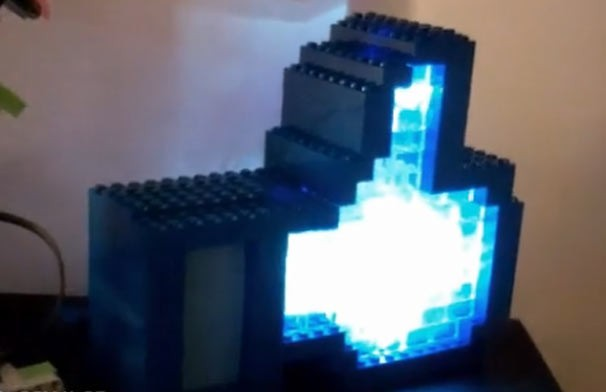
\includegraphics[scale=0.85]{img/prestudies-likehand}
\caption{LikeLight from Red Pepper Labs\cite{link:likelight}}
\label{fig:prestudies-likehand}
\end{figure}

\newpage

\section{Our own ideas}

\subsection{YepMailbox}
The YepMailbox (Figure \ref{fig:prestudies-YepMailbox}) was another concept of a tangible Arduino-powered prototype 
that would interact with the user Facebook wall. The mail flag would rise powered by a small servo motor and a printer 
would print out the new message.

\begin{figure}[h!]
\centering 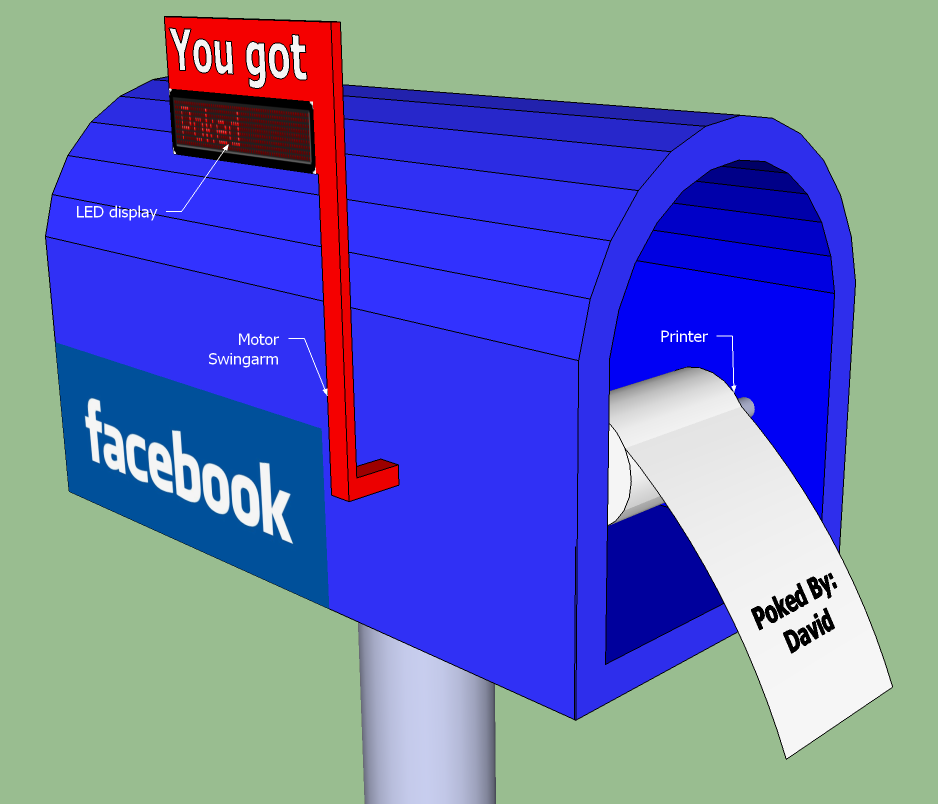
\includegraphics[scale=0.4]{img/prestudies-YepMailbox}
\caption{Our concept idea of the YepMailbox}
\label{fig:prestudies-YepMailbox}
\end{figure}

\newpage

\subsection{Facebook Wall}
The "Facebook Wall" (Figure \ref{fig:prestudies-facebookwall}) is a wall with two holes in it for people to put their faces in.
The prototype would then make a picture and replace the wall with some image and add bodies to the two faces. The image 
would then be automatically uploaded and posted on Facebook.

\begin{figure}[h!]
\centering 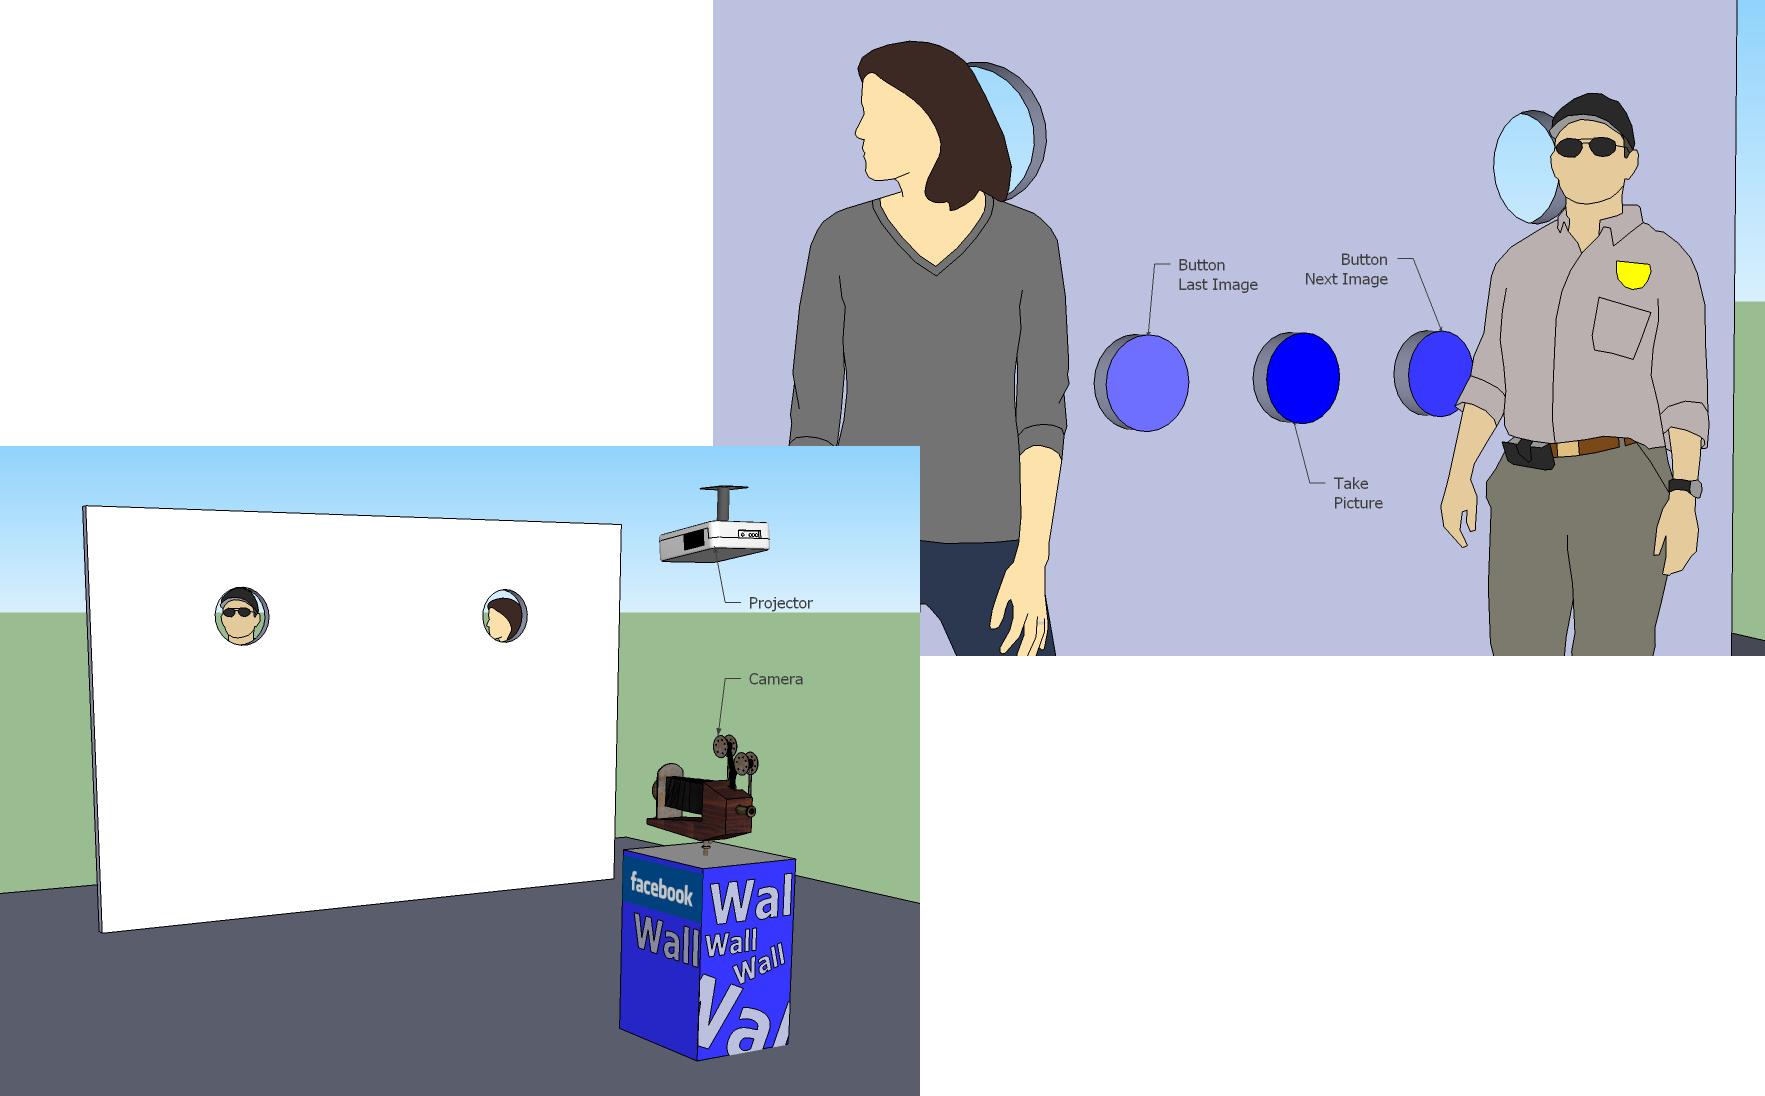
\includegraphics[scale=0.22]{img/prestudies-facebookwall}
\caption{Our concept idea of the Facebook Wall}
\label{fig:prestudies-facebookwall}
\end{figure}

\newpage

\subsection{T-Shirt}
The T-Shirt (Figure \ref{fig:prestudies-tshirt})  features electronic circuits powered by an Arduino Lilypad board.
The Lilypad is an Arduino board designed especially to be wore. It is connected wirelessly to the Internet through
an Android phone, and downloads status updates from a social network such as Facebook.
The content fetched is then displayed through one of the electronic devices: LEDs, LCD screen,
sound module or a vibration module.


\begin{figure}[h!]
\centering 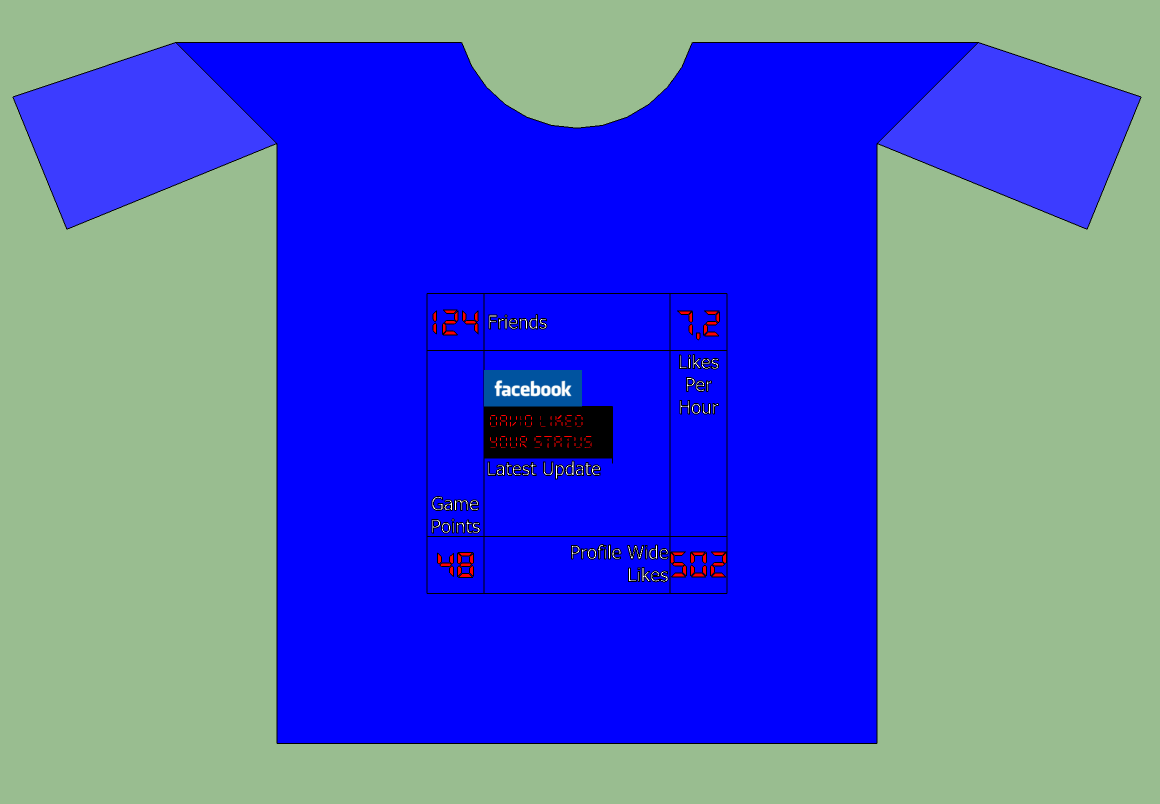
\includegraphics[scale=0.35]{img/prestudies-tshirt}
\caption{Our first concept idea of the T-shirt prototype}
\label{fig:prestudies-tshirt}
\end{figure}

\newpage

\section{Conclusion}
We presented our various ideas and concepts to the customer and let him decide on what he would
like the group to work on. The client liked the t-shirt idea, and he decided that it would be the main prototype for this project. 
After some iterations the t-shirt got swapped out with a jacket due to practical reasons for implementing the hardware. 
The prototypes work as proof-of-concept that our developer libraries function as they should and work as the same time as an 
example on how the libraries can be used. In our example we show how you can connect social networks (Twitter, Facebook, etc.) to 
tangible Arduino interfaces (LED, buzzer, sound, buttons, etc.). The customer requested one or two additional smaller prototypes in 
addition to the oSNAP Jacket to prove that our libraries can be successfully used to develop different prototypes. Each of the prototypes are 
described in more detail in section \ref{sec:prototypes}.
